\part{Diagramme de collaboration - Validation de l'architecture globale}
\setcounter{section}{0}

\section{Diagramme de collaboration}
\begin{figure}[H]
\noindent\makebox[\textwidth]{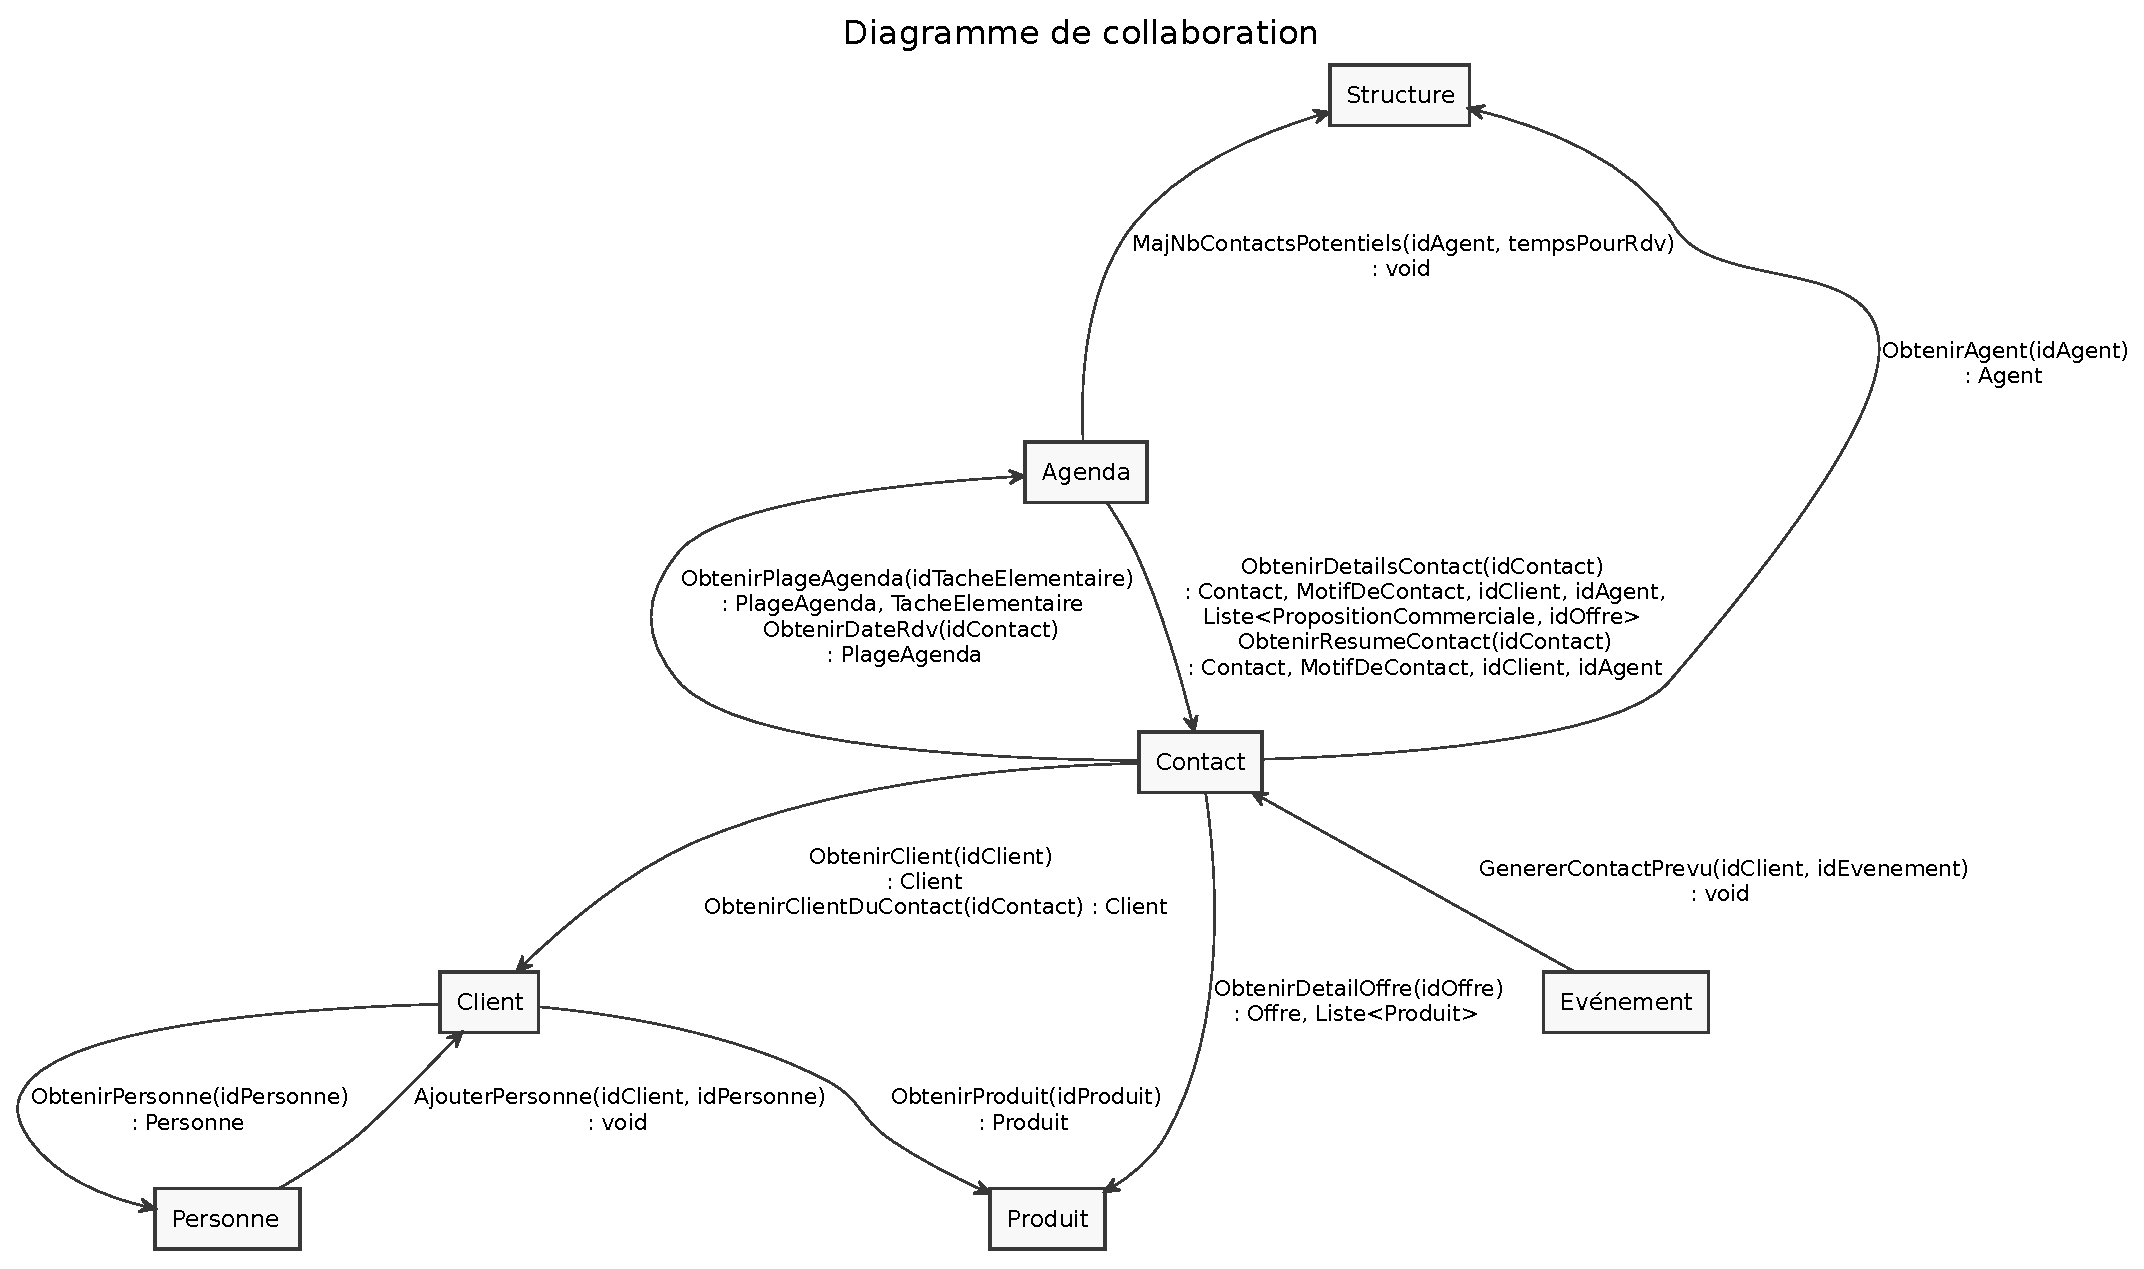
\includegraphics[width=23cm, angle=90]{figures/eps/collaboration.eps}}
\caption{Diagramme de collaboration}
\end{figure}

On constate que la répartition des services entre les blocs est centrée autour de l'objet contact, ce qui est logique, puisqu'il s'agit du coeur de métier du projet. Autrement, la répartition des différents appels semble être assez homogène, et on n'observe pas de redondances.\\

Sinon, on note qu'il y a essentiellement des services de consultation et quelques services de modification. \\ 
Enfin, on observe qu'on retrouve les liens établies dans le MCD dans le diagramme de collaboration (exemple : entre contact et client, ou client et personne). 



